\documentclass{beamer}
\usetheme{tokitex}

\usepackage{graphics}
\usepackage{multirow}
\usepackage{tabto}

\usepackage[english,bahasa]{babel}
\newtranslation[to=bahasa]{Section}{Bagian}
\newtranslation[to=bahasa]{Subsection}{Subbagian}

\usepackage{listings, lstautogobble}
\usepackage{color}

\definecolor{dkgreen}{rgb}{0,0.6,0}
\definecolor{gray}{rgb}{0.5,0.5,0.5}
\definecolor{mauve}{rgb}{0.58,0,0.82}

\lstset{frame=tb,
  language=pascal,
  aboveskip=1mm,
  belowskip=1mm,
  showstringspaces=false,
  columns=fullflexible,
  keepspaces=true,
  basicstyle={\small\ttfamily},
  numbers=none,
  numberstyle=\tiny\color{gray},
  keywordstyle=\color{blue},
  commentstyle=\color{dkgreen},
  stringstyle=\color{mauve},
  breaklines=true,
  breakatwhitespace=true,
  autogobble=true
}

\title{Divide and Conquer}
\author{Tim Olimpiade Komputer Indonesia}
\date{}

\begin{document}

\begin{frame}
\titlepage
\end{frame}

\begin{frame}
\frametitle{Pengenalan}
\begin{itemize}
  \item Kadang permasalahan lebih mudah diselesaikan jika dibagi menjadi beberapa masalah yang lebih kecil.
  \item Masalah lebih kecil kemudian diselesaikan secara independen.
  \item Hasilnya digabungkan menjadi solusi untuk masalah yang lebih besar.
  \item Strategi ini digunakan Belanda pada masa penjajahan, biasa dipelajari sebagai \foreignTerm{divide et impera}.
\end{itemize}
\end{frame}

\begin{frame}
\frametitle{Konsep}
Secara umum, \foreignTerm{divide and conquer} terdiri dari tiga tahap:
\begin{itemize}
  \item \newTerm{Divide}: membagi masalah yang besar menjadi masalah yang lebih kecil.
  \item \newTerm{Conquer}: ketika masalah sudah cukup kecil untuk diselesaikan, langsung selesaikan.
  \item \newTerm{Combine}: menggabungkan solusi dari masalah-masalah yang lebih kecil menjadi solusi untuk masalah yang besar.
\end{itemize}
\end{frame}

\begin{frame}
\frametitle{Ilustrasi Konsep}
\begin{figure}
  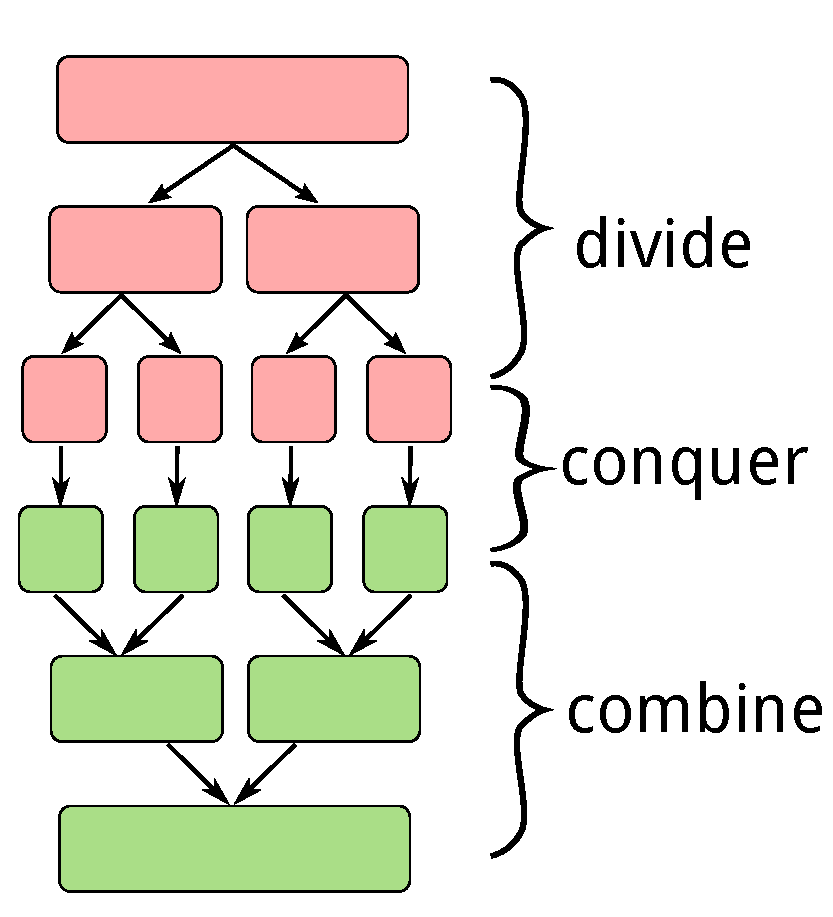
\includegraphics[width=6.5cm]{asset/dnc-concept.pdf}
\end{figure}
\end{frame}

\begin{frame}
\frametitle{Studi Kasus 1: Merge Sort}
\foreignTerm{Merge Sort}: algoritma pengurutan O($N \log{N}$).
\newline
\newline
Prinsip kerja algoritma ini adalah:
\begin{itemize}
  \item \foreignTerm{Divide}: jika array yang akan diurutkan berukuran besar, bagi menjadi dua array sama besar.
  \item \foreignTerm{Conquer}: ketika array sudah cukup kecil untuk diurutkan, lakukan pengurutan.
  \item \foreignTerm{Combine}: dari dua array yang telah terurut, gabungkan menjadi sebuah array terurut.
\end{itemize}
\end{frame}

\begin{frame}
\frametitle{Contoh Eksekusi Merge Sort}
Kapan suatu array dianggap cukup kecil untuk dapat diurutkan secara langsung?
\newline
\begin{itemize}
  \item Sederhana, yaitu ketika panjang array itu tinggal \emph{satu}.
  \item Tentu saja, array dengan panjang satu \emp{sudah pasti} terurut.
  \newline
\end{itemize}
Jadi selama array yang hendak diurutkan masih memiliki panjang lebih dari satu, bagi array itu menjadi dua.
\end{frame}

\begin{frame}
\frametitle{Contoh Eksekusi Merge Sort (lanj.)}
Array yang dimiliki masih terlalu besar, belah menjadi dua.
\begin{figure}
  \centering
  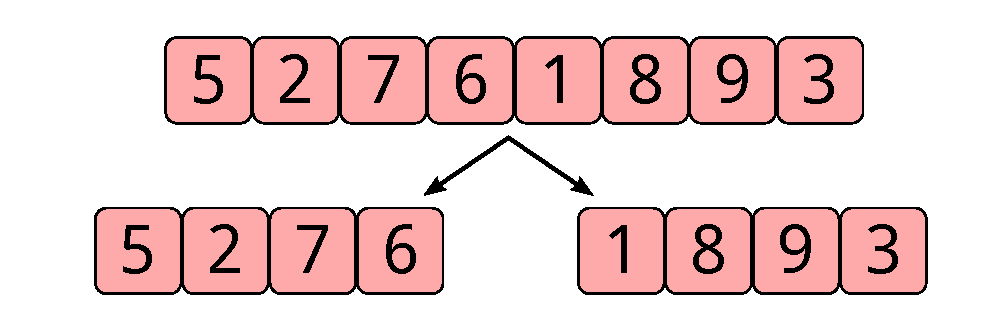
\includegraphics[width=10 cm]{asset/merge-sort-demo-1.pdf}
\end{figure}
\end{frame}

\begin{frame}
\frametitle{Contoh Eksekusi Merge Sort (lanj.)}
Masih belum cukup kecil, belah lagi.
\begin{figure}
  \centering
  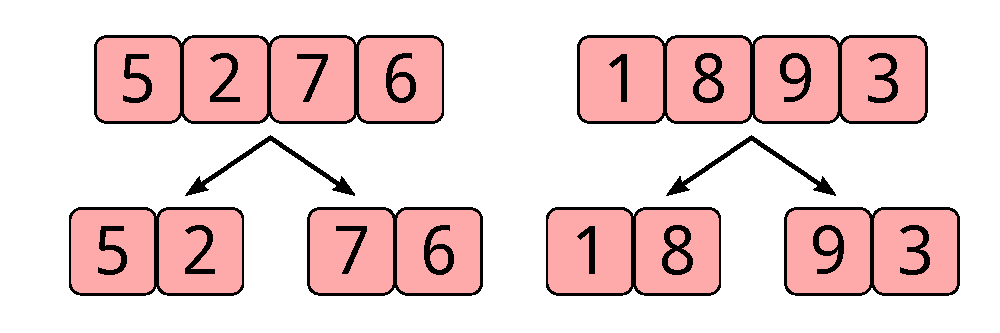
\includegraphics[width=10 cm]{asset/merge-sort-demo-2.pdf}
\end{figure}
\end{frame}

\begin{frame}
\frametitle{Contoh Eksekusi Merge Sort (lanj.)}
Masih belum cukup kecil, belah lagi.
\begin{figure}
  \centering
  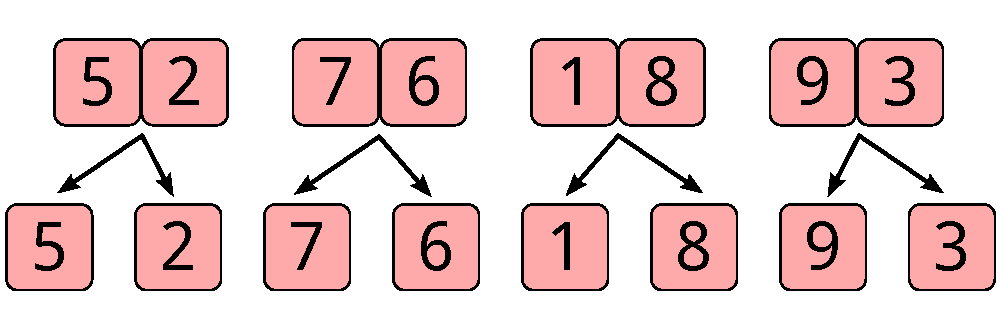
\includegraphics[width=10 cm]{asset/merge-sort-demo-3.pdf}
\end{figure}
\end{frame}

\begin{frame}
\frametitle{Contoh Eksekusi Merge Sort (lanj.)}
Kini kita memiliki "array" yang panjangnya hanya satu.\newline

Secara definisi, "array" ini telah terurut.
\begin{figure}
  \centering
  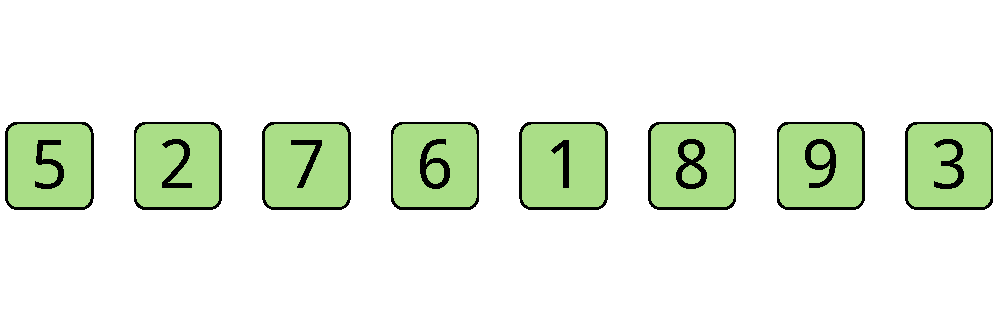
\includegraphics[width=10 cm]{asset/merge-sort-demo-4.pdf}
\end{figure}
\end{frame}

\begin{frame}
\frametitle{Contoh Eksekusi Merge Sort (lanj.)}
Gabungkan hasil pembelahan sebelumnya.
\begin{figure}
  \centering
  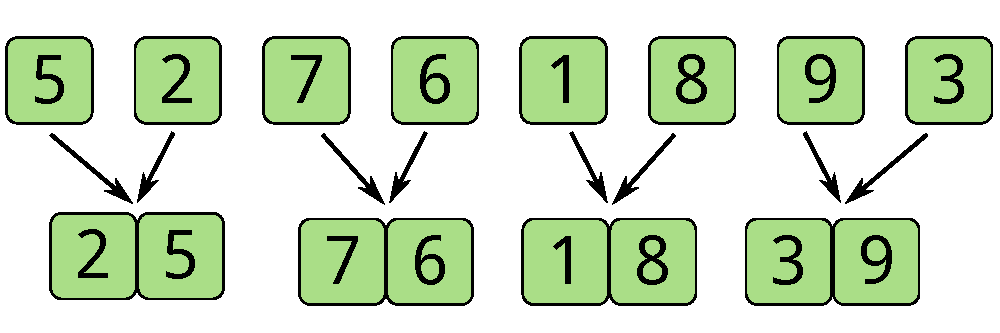
\includegraphics[width=10 cm]{asset/merge-sort-demo-5.pdf}
\end{figure}
\end{frame}

\begin{frame}
\frametitle{Contoh Eksekusi Merge Sort (lanj.)}
Gabungkan lagi.
\begin{figure}
  \centering
  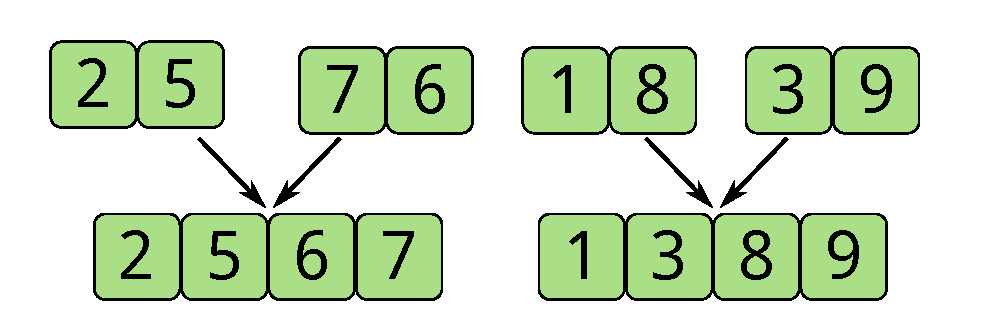
\includegraphics[width=10 cm]{asset/merge-sort-demo-6.pdf}
\end{figure}
\end{frame}

\begin{frame}
\frametitle{Contoh Eksekusi Merge Sort (lanj.)}
Gabungkan lagi dan akhirnya didapatkan array terurut.
\begin{figure}
  \centering
  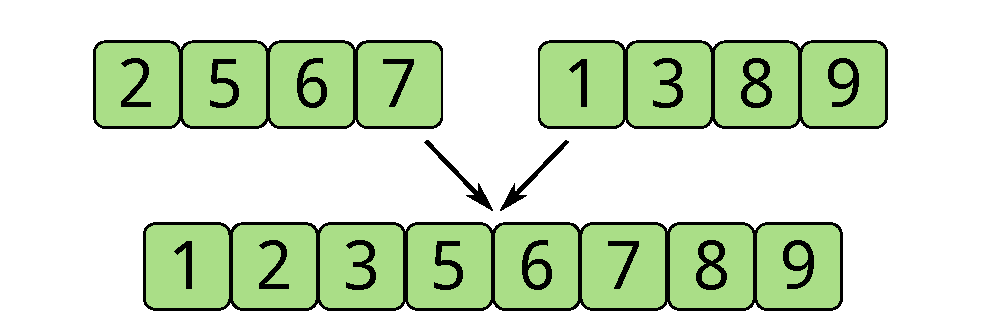
\includegraphics[width=10 cm]{asset/merge-sort-demo-7.pdf}
\end{figure}
\end{frame}

\begin{frame}
\frametitle{Menggabungkan Dua Array Terurut}
Bagaimana cara menggabungkan dua array yang telah terurut?
\begin{figure}
  \centering
  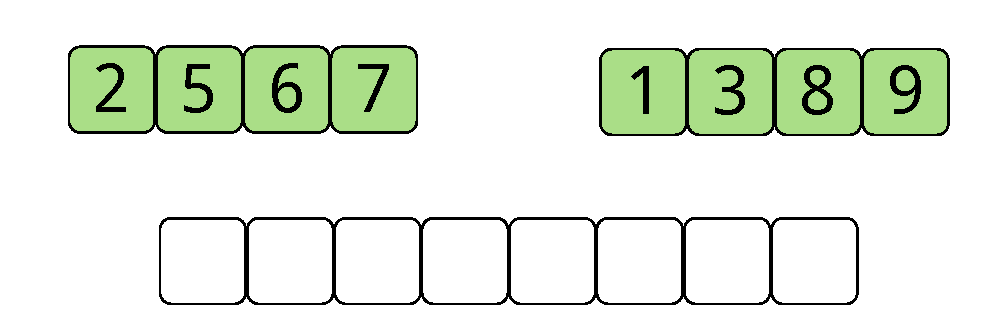
\includegraphics[width=10 cm]{asset/merge-array-pair-1.pdf}
\end{figure}
\end{frame}

\begin{frame}
\frametitle{Menggabungkan Dua Array Terurut (lanj.)}
Observasi: elemen terkecil dari array gabungan pasti salah satu dari elemen terkecil array yang terurut. Lebih tepatnya, yang memiliki nilai lebih kecil.
\begin{figure}
  \centering
  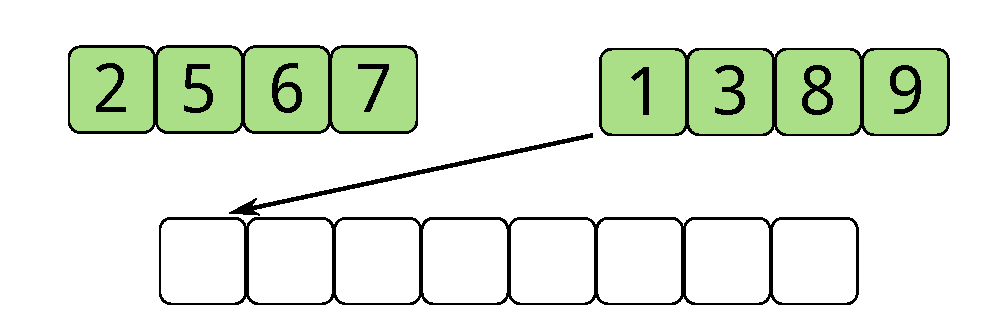
\includegraphics[width=10 cm]{asset/merge-array-pair-2.pdf}
\end{figure}
\end{frame}

\begin{frame}
\frametitle{Menggabungkan Dua Array Terurut (lanj.)}
Ulangi hal serupa sampai salah satu atau kedua array habis.

\begin{figure}
  \centering
  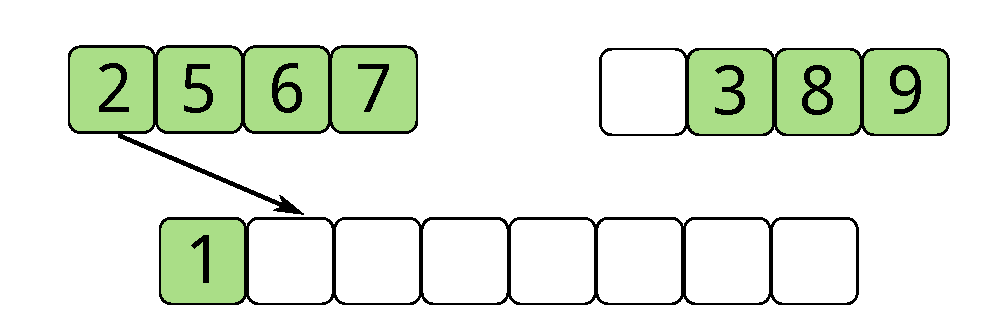
\includegraphics[width=10 cm]{asset/merge-array-pair-3.pdf}
\end{figure}
\end{frame}

\begin{frame}
\frametitle{Menggabungkan Dua Array Terurut (lanj.)}
\begin{figure}
  \centering
  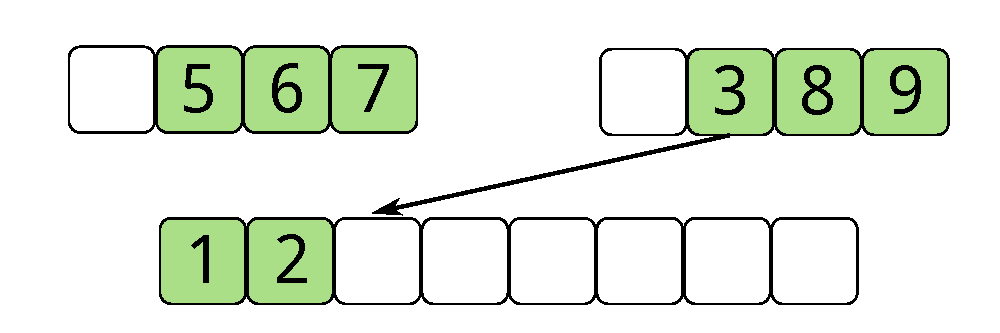
\includegraphics[width=10 cm]{asset/merge-array-pair-4.pdf}
\end{figure}
\end{frame}

\begin{frame}
\frametitle{Menggabungkan Dua Array Terurut (lanj.)}
\begin{figure}
  \centering
  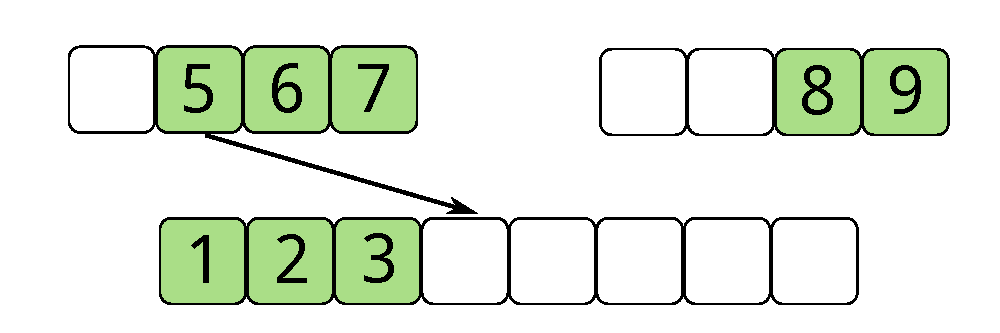
\includegraphics[width=10 cm]{asset/merge-array-pair-5.pdf}
\end{figure}
\end{frame}

\begin{frame}
\frametitle{Menggabungkan Dua Array Terurut (lanj.)}
\begin{figure}
  \centering
  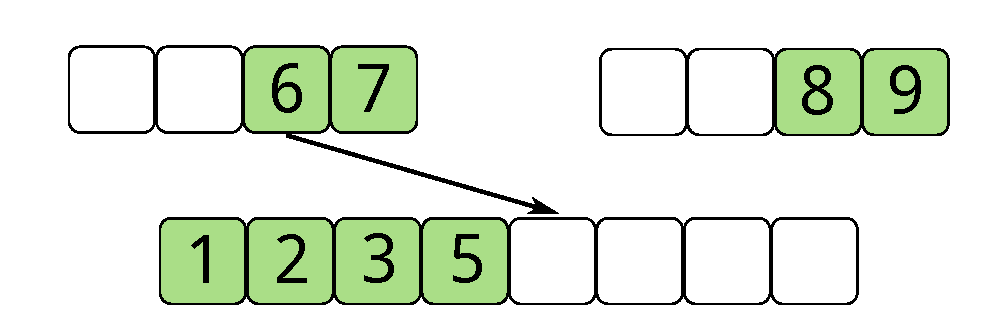
\includegraphics[width=10 cm]{asset/merge-array-pair-6.pdf}
\end{figure}
\end{frame}

\begin{frame}
\frametitle{Menggabungkan Dua Array Terurut (lanj.)}
\begin{figure}
  \centering
  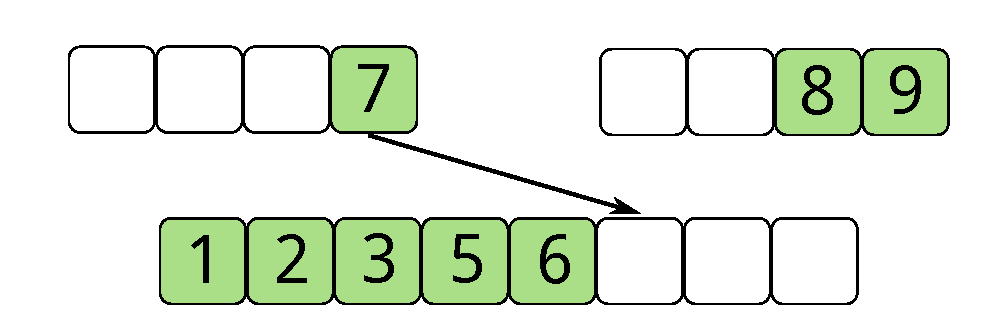
\includegraphics[width=10 cm]{asset/merge-array-pair-7.pdf}
\end{figure}
\end{frame}

\begin{frame}
\frametitle{Menggabungkan Dua Array Terurut (lanj.)}
Ketika salah satu array telah habis, array yang masih bersisa tinggal ditempelkan di akhir array gabungan.
\begin{figure}
  \centering
  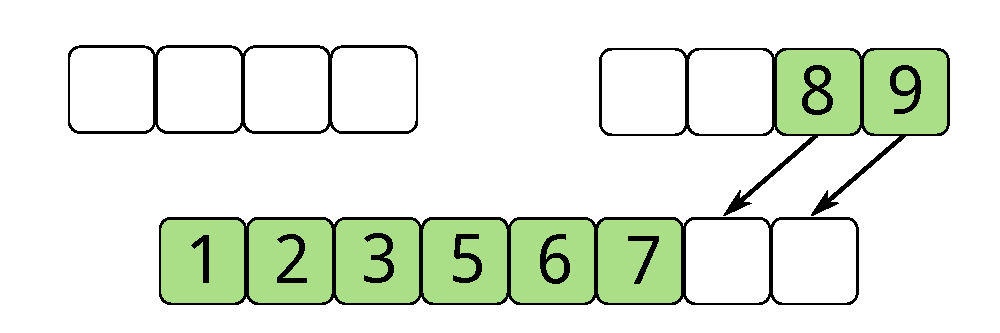
\includegraphics[width=10 cm]{asset/merge-array-pair-8.pdf}
\end{figure}
\end{frame}

\begin{frame}
\frametitle{Menggabungkan Dua Array Terurut (lanj.)}
Selesai proses menggabungkan.
\begin{figure}
  \centering
  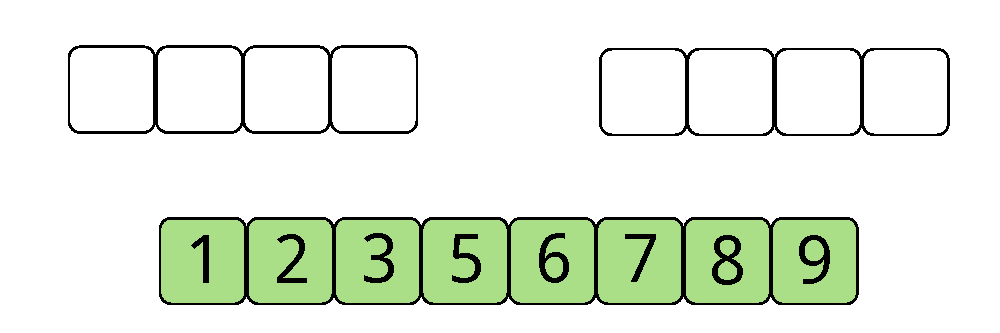
\includegraphics[width=10 cm]{asset/merge-array-pair-9.pdf}
\end{figure}
\end{frame}

\begin{frame}
\frametitle{Analisis Menggabungkan Dua Array Terurut}
\begin{itemize}
  \item Misalkan kedua array terurut yang akan digabung adalah $A$ dan $B$.
  \item Pada setiap langkah, salah satu dari elemen $A$ atau $B$ dipindahkan.
  \item Total terdapat $|A| + |B|$ proses, sehingga kompleksitasnya $O(|A| + |B|)$.
\end{itemize}
\end{frame}

\begin{frame}
\frametitle{Analisis Algoritma Merge Sort}
\begin{itemize}
  \item Misalkan $N$ menyatakan ukuran dari array.
  \item Dengan sifat membagi dua secara terus-menerus, kedalaman rekursif dari Merge Sort adalah $O(\log{N})$
  \item Untuk setiap kedalaman, dilakukan aktivitas \foreignTerm{divide} dan \foreignTerm{combine}.
  \item \foreignTerm{Divide} dan \foreignTerm{conquer} selalu bekerja dalam $O(1)$.
\end{itemize}
\end{frame}

\begin{frame}
\frametitle{Analisis Algoritma Merge Sort (lanj.)}
\begin{figure}
  \centering
  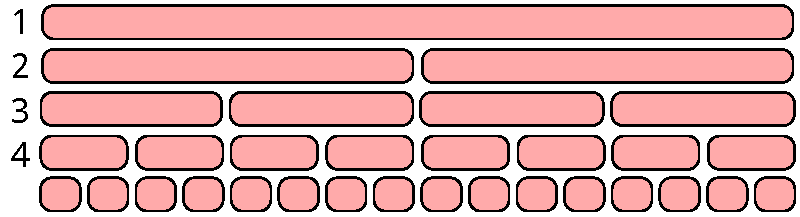
\includegraphics[width=10 cm]{asset/merge-sort-complexity.pdf}
\end{figure}
\begin{itemize}
  \item Kedalaman 1, proses \foreignTerm{combine} bekerja dalam $O(2 \times \frac{N}{2})$
  \item Kedalaman 2, proses \foreignTerm{combine} bekerja dalam $O(4 \times \frac{N}{4})$
  \item Kedalaman 3, proses \foreignTerm{combine} bekerja dalam $O(8 \times \frac{N}{8})$  
  \item ...  
\end{itemize}
\end{frame}

\begin{frame}
\frametitle{Analisis Algoritma Merge Sort (lanj.)}
\begin{itemize}
  \item Mudah untuk disadari bahwa keseluruhan proses untuk setiap kedalaman bekerja dalam $O(N)$.
  \item Karena kedalaman maksimal adalah $O(\log{N})$, kompleksitas akhir \foreignTerm{Merge Sort} adalah $O(N \log{N})$.
  \item Jauh lebih cepat dari algoritma pengurutan $O(N^2)$ seperti \foreignTerm{Bubble Sort}.
  \item \foreignTerm{Merge Sort} mampu mengurutkan array dengan ratusan ribu elemen dalam waktu singkat.
\end{itemize}
\end{frame}

%\begin{frame}
%\frametitle{Perbandingan Algoritma Pengurutan}
%TODO: grafik keren
%\end{frame}

\begin{frame}
\frametitle{Contoh Implementasi}
Mengurutkan $arr[left..right]$:
\noindent\rule{10cm}{0.4pt}
\begin{codebox}
\Procname{$\proc{mergeSort}(arr[], left, right)$}
\li \If $left \isequal right$ \Then
\li   \Comment Tinggal 1 elemen, sudah pasti terurut
\li \Else 
\li   $mid \gets (left + right)$ div $2$
\li   $\proc{mergeSort}(arr, left, mid)$
\li   $\proc{mergeSort}(arr, mid+1, right)$
\li   $\proc{merge}(arr, left, mid, mid+1, right)$
    \End
\end{codebox}
\end{frame}

% WARNING: baris-baris ininn menggunakan perintah setcounter
% PASTIKAN ANDA MENGUBAHNYA JIKA ANDA MENGUBAH PSEUDOCODE
\begin{frame}
\frametitle{Contoh Implementasi (lanj.)}
Menggabungkan $arr[aLeft..aRight]$ dengan $arr[bLeft..bRight]$ yang telah terurut:
\noindent\rule{10cm}{0.4pt}
\begin{codebox}
\Procname{$\proc{merge}(arr[], aLeft, aRight, bLeft, bRight)$}
\li \Comment Buat array penampungan sementara bernama $temp$
\li \Comment Isikan $temp[aLeft \twodots bRight]$ dengan nilai dari $arr[aLeft \twodots bRight]$
\li $tIndex \gets 1$
\li $aIndex \gets aLeft$
\li $bIndex \gets bLeft$
\li $...$
\end{codebox}
\end{frame}

% WARNING: baris-baris ininn menggunakan perintah setcounter
% PASTIKAN ANDA MENGUBAHNYA JIKA ANDA MENGUBAH PSEUDOCODE
\begin{frame}
\frametitle{Contoh Implementasi (lanj.)}
\begin{codebox}
\setcounter{codelinenumber}{4}
\li $...$
\li \Comment Selama kedua subarray masih ada isinya, ambil yang terkecil
\li \While $(aIndex \leq aRight)$ and $(bIndex \leq bRight)$ \Do
\li   \If $temp[aIndex] < temp[bIndex]$ \Then
\li     $arr[tIndex] \gets temp[aIndex]$
\li     $aIndex \gets aIndex + 1$
\li   \Else
\li     $arr[tIndex] \gets temp[bIndex]$
\li     $bIndex \gets bIndex + 1$
      \End
\li   $tIndex \gets tIndex + 1$
    \End
\li $...$
\end{codebox}
\end{frame}

% WARNING: baris-baris ininn menggunakan perintah setcounter
% PASTIKAN ANDA MENGUBAHNYA JIKA ANDA MENGUBAH PSEUDOCODE
\begin{frame}
\frametitle{Contoh Implementasi (lanj.)}
\begin{codebox}
\setcounter{codelinenumber}{13}
\li $...$
\li \Comment Masukkan subarray yang masih bersisa
\li \Comment Hanya salah satu dari kedua while ini yang akan dieksekusi
\li \While $(aIndex \leq aRight)$ \Do
\li   $arr[tIndex] \gets temp[aIndex]$
\li   $aIndex \gets aIndex + 1$
\li   $tIndex \gets tIndex + 1$
    \End
\li \While $(bIndex \leq bRight)$ \Do
\li   $arr[tIndex] \gets temp[bIndex]$
\li   $bIndex \gets bIndex + 1$
\li   $tIndex \gets tIndex + 1$
    \End
\li \Comment selesai penggabungan
\end{codebox}
\end{frame}

%\begin{frame}[fragile]
%\frametitle{Analisis Merge Sort Secara Rekursif}
%\begin{itemize}
%  \item Umumnya \foreignTerm{Divide and Conquer} memiliki sifat rekursif secara alami.
%  \item Misalkan kita selalu membagi masalah menjadi dua, maka bentuk umumnya:
%  
%\begin{lstlisting}
%solve(problem)
%  if (problem cukup kecil)
%    return conquer(problem)
%  else
%    [subproblem1, subproblem2] := divide(problem)
%    
%    solve(subproblem1)
%    solve(subproblem2)
%    
%    return combine(subproblem1, subproblem2)
%\end{lstlisting}
%\end{itemize}
%\end{frame}
%
%\begin{frame}
%\frametitle{Analisis Merge Sort Secara Rekursif (lanj.)}
%\begin{itemize}
%  \item Analisis algoritma juga dapat dilakukan secara rekursif.
%  \item Misalkan $T(N)}$ menyatakan kompleksitas 
%\end{itemize}
%\end{frame}

\begin{frame}
\frametitle{Studi Kasus 2: Mencari Nilai Terbesar}
\begin{itemize}
  \item Diberikan sebuah array $A$ yang memiliki $N$ bilangan.
  \item Cari nilai terbesar yang ada pada $A$!\newline
  \item Masalah ini mudah diselesaikan dengan perulangan biasa.
  \item Namun coba kita selesaikan dengan \foreignTerm{divide and conquer}.\end{itemize}
\end{frame}

\begin{frame}
\frametitle{Studi Kasus 2: Mencari Nilai Terbesar (lanj.)}
Pertama kita definisikan tahap-tahapnya:
\begin{itemize}
  \item \foreignTerm{Divide}: jika array berukuran besar, bagi menjadi dua subarray.
  \item \foreignTerm{Conquer}: ketika array hanya berisi satu elemen, nilai terbesarnya pasti elemen tersebut.
  \item \foreignTerm{Combine}: nilai terbesar dari array adalah maksimum dari nilai terbesar di subarray pertama dan nilai terbesar di subarray kedua.
\end{itemize}
\end{frame}

\begin{frame}
\frametitle{Contoh Implementasi}
\begin{codebox}
\Procname{$\proc{findMax}(arr[], left, right)$}
\li \If $left \isequal right$ \Then
\li   \Return $arr[left]$
\li \Else 
\li   $mid \gets (left + right)$ div $2$
\li   $leftMax \gets \proc{findMax}(arr, left, mid)$
\li   $rightMax \gets \proc{findMax}(arr, mid+1, right)$
\li   \Return $\func{max}(leftMax, rightMax)$
    \End
\end{codebox}
\end{frame}

\begin{frame}
\frametitle{Analisis Algoritma Mencari Nilai Terbesar}
\begin{figure}
  \centering
  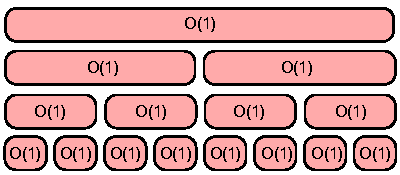
\includegraphics[width=8 cm]{asset/find-max-complexity.pdf}
\end{figure}
\begin{itemize}
  \item Setiap operasi \foreignTerm{divide}, \foreignTerm{conquer}, dan \foreignTerm{combine} bekerja dalam $O(1)$.
  \item Ketiga operasi tersebut dilaksanakan sebanyak\\1 + 2 + 4 + 8 + ... + $2^L$ kali, dengan $2^L$ mendekati $N$.
  \item Sehingga totalnya dilaksanakan sekitar $2^{L+1} - 1 = 2N$ operasi.
\end{itemize}
\end{frame}

\begin{frame}
\frametitle{Analisis Algoritma Mencari Nilai Terbesar (lanj.)}
\begin{itemize}
  \item Kompleksitas akhirnya adalah $O(N)$.
  \item Ternyata strategi ini tidak lebih baik dari mencari nilai maksimum satu per satu
\end{itemize}
\end{frame}

\begin{frame}
\frametitle{Penutup}
\begin{itemize}
  \item \foreignTerm{Divide and Conquer} merupakan salah satu strategi dalam penyelesaian masalah.
  \item Konsep ini banyak digunakan pada struktur data lanjutan dan komputasional geometri.
  \item Jika suatu masalah dapat dibelah menjadi beberapa masalah yang lebih kecil dan serupa, kemudian hasil dari masing-masing penyelesaiannya dapat digabungkan, maka \foreignTerm{Divide and Conquer} dapat digunakan.
\end{itemize}
\end{frame}

\end{document}
